\section{The invasion scale and the voter endpoint}
\label{sec:line}
\subsection{Parameter survey}
\label{sec:phase}

The earlier strip survey gives a nonmonotonic invasion scale
(Fig.~\ref{fig:phase}; Supplemental Table~\ref{S-tab:line}). Starting
from the exceptional $p=0$ reference, it reaches a maximum near
$p=0.25$--0.5 and decreases toward $(p,q)=(1,0)$.
Over the sampled near-voter range it is approximately
$q^*\simeq0.25\alpha(1-p)$. The $p=0$ model has extra frozen states,
so that datum is not a measured $p\to0^+$ limit.
The survey densities were measured at specified probabilities and
observation windows; they are not extrapolated jumps.
In particular, the historical $p=0.99$ and 0.995 points are marked
separately in the figure. At the latter point, longer runs overturn
the apparent stationarity.

\begin{figure}
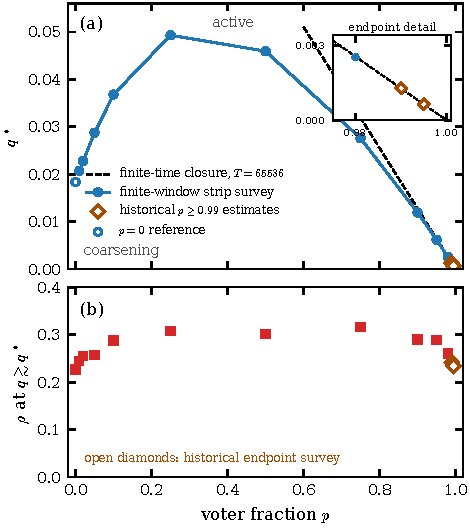
\includegraphics[width=\columnwidth]{figs/fig_phase}
\caption{(a) Finite-window invasion survey at $\alpha=1/2$ from strip
fronts (Table~\ref{S-tab:line}), with the refined $p=1/2$ operational
reference. The open blue circle denotes the $p=0$ reference with
additional frozen states. Open orange diamonds identify the historical
$p=0.99$ and 0.995 estimates; the inset enlarges the endpoint region.
The dashed line is the finite-time closure
$q_f(T)=c_f(T)\alpha(1-p)$ at $T=65536$, where $c_f=0.2553$.
(b) Time-weighted density at the actual nearby probabilities $q_\rho$
in Table~\ref{S-tab:line}, with equal run weights and one standard error.
Open orange diamonds again mark the historical endpoint survey.
The $p\ge0.99$ summaries combine nearby probabilities and observation
horizons. Longer trajectories at $p=0.995$, $q=0.000640$ show substantial
late decay in Fig.~\ref{fig:gpu_near20m}; the historical endpoint markers
do not locate a limiting transition or its density jump.}
\label{fig:phase}
\end{figure}


\subsection{Longer times reveal continuing relaxation}
\label{sec:voter}

At $p=0.995$, $q=0.000640$, four $L=8192$ trajectories run to
$2\times10^7$ steps have unconditional mean density 0.189 over
$5$--$10\times10^6$ and 0.122 over $10$--$20\times10^6$; one reaches
consensus. At $q=0.000642$ all four remain active, with late mean 0.2204,
but their paired changes between the two halves of the last window are
$-0.00154$, $-0.00578$, $-0.00155$, and $-0.00971$.
The mean change is $-0.00464$. Its percentile-bootstrap interval is
$[-0.0077,-0.0015]$, whereas a normal-reference paired $t_3$ interval
is $[-0.0109,+0.0016]$. The common sign is an observation about these
four runs; it is not a method-independent precision statement about
the population mean drift.
At $q=0.000644$ and 0.000648, the late means are 0.2265 and 0.2326,
with no consistent drift resolved over the same window.

\begin{figure*}
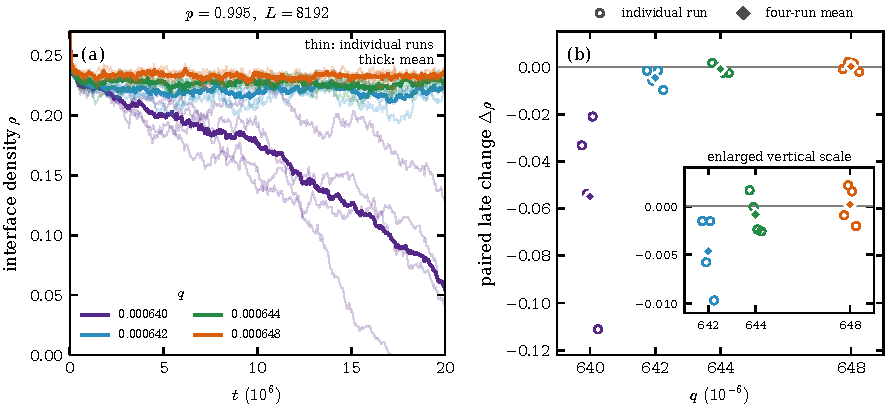
\includegraphics[width=\textwidth]{figs/fig_gpu_near20m}
\caption{Largest-system time dependence near the voter point,
$p=0.995$, $\alpha=1/2$, and $L=8192$. All four declared independent
runs at each $q=0.000640$, 0.000642, 0.000644, and 0.000648 are followed
to $T=2\times10^7$. (a) Thin curves show the individual trajectories
and thick curves their equal-run means. The trajectory that reaches
consensus at $q=0.000640$ contributes its known zero activity thereafter.
(b) Open circles show each run's time-weighted mean density over
$15$--$20\times10^6$ minus that over $10$--$15\times10^6$; diamonds
show the four-run means. Horizontal offsets separate the four runs
visually. The inset repeats the three higher-$q$ groups on an enlarged
vertical scale. The midpoint cohort at $q=0.000642$ was declared
independently after the original grid. The displayed run variation
does not assign a calibrated confidence level or establish stationarity.}
\label{fig:gpu_near20m}
\end{figure*}


The fronts reinforce the distinction between persistence and a measured
coexistence boundary. At $q=0.000640$ the strip interior decays strongly,
and only one of four runs keeps separated-front geometry over
$5$--$10\times10^6$ steps. Fitting its envelope would conflate invasion
with internal loss of activity. The higher-$q$ bands retain activity but
can encounter the finite box. These data do not locate a late stationary
front at the smallest probabilities (Supplemental Sec.~\ref{S-sec:svoter}).

Small seeds provide another finite-time diagnostic. At $p=0.99$,
$q=0.0012954$, a separately declared ensemble of eight million seeds
has 19 survivors and no boundary escapes at $t=10^6$. Counts fall from
793 to 97 between $t=63096$ and 251189, giving an effective survival
exponent of 1.52; the last sufficiently populated factor-four window
gives 1.26 with an interval including one. This quantifies strong
transient suppression at a specified probability.
A nonlinear voter model need not obey a voter asymptote before its
crossover~\cite{castellano2012,azizi2020}; the seed experiment therefore
does not locate criticality or establish survival at infinite time.
Magnetic size ratios and active-wall observations are also restricted
to their sampled points. None excludes an unsampled Ising--DP interval.

Reducing each site's update probability to $r=1/2,1/4,1/8$ changes
the measured invasion scale while retaining finite-time active and
front signatures (Supplemental Sec.~\ref{S-sec:async}). This tests
robustness to reduced synchrony. A strict continuous-time result would
require the $r\to0$ limit at fixed physical time $rt$.
The asymptotic transition order near the voter endpoint remains open.
